\documentclass[11pt,a4paper,twoside]{article}
\usepackage{a4wide}	% für gut definierte Seitenränder und Platzausnutzung
\usepackage[utf8]{inputenc}	% für Umlaute
\usepackage{amssymb,amsmath}
\usepackage{booktabs}   % schöne Tabellen
\usepackage[pdftex]{graphicx}
\graphicspath{{./pic/}}
\usepackage{epstopdf}
\usepackage{siunitx}	% für SI-Einheiten; siehe http://mirror.unicorncloud.org/CTAN/macros/latex/contrib/siunitx/siunitx.pdf
\usepackage[version=3]{mhchem}	% chemische Symbole mit \ce{}
\usepackage{listings} 	% für Einbinden von Quellcode
\usepackage{minted}     % Johannes Lieblingspackage für Quellcode
\usepackage{color}	% für das Einfärben von eingebundenem Quellcode
\usepackage{longtable}	% für das Erstellen mehrseitiger Tabellen
\usepackage[german]{isodate} % Datumformatierung für \today
\usepackage{marvosym}
\usepackage{ulem}	% 

% declaring custom units
\DeclareSIUnit \mag {mag}
\DeclareSIUnit \parsec {pc}
\DeclareSIUnit \AU {AU}
\DeclareSIUnit \pixel {pixel}

% format angle display
\sisetup{add-arc-degree-zero}
\sisetup{add-arc-minute-zero}
\sisetup{add-arc-second-zero}
\sisetup{arc-separator = \,}


%Befehl, um Quellcode einzufügen: 
%\lstinputlisting[caption = {``title``}, captionpos = b, language=C++]{data.cpp}

%Befehl, um Graphik einzufügen:   
%\begin{figure}
%  \centering
%  \includegraphics[width=0.7\textwidth, angle=-90]{center_diff.eps}
%  \caption{centered differencing at t = 4}
%\end{figure}

% Befehl für kein ``\noindent mehr''
\setlength\parindent{0pt}

%\lstset{numbers=left}

\newcommand{\op}[1]{\operatorname{#1}}

% Konsistente Variablennamen:
\newcommand{\zen}{\ensuremath{\nu} }    % zenith angle
\newcommand{\hei}{\ensuremath{h} }      % height angle
\newcommand{\HA}{\ensuremath{\Gamma} }  % hour angle \HA
\newcommand{\DEC}{\ensuremath{\delta} } % declination \DE
\newcommand{\LAT}{\ensuremath{\Phi} }   % latitude \LAT
\newcommand{\electron}{\ce{e^-}}
\newcommand{\SNR}{\ensuremath{\frac{S}{N}} }

\newcommand{\MgFe}{\ensuremath{[\text{MgFe}]^\prime} }
\newcommand{\ZH}{\ensuremath{[\text{Z}/\text{H}]} }
\newcommand{\Hbo}{\ensuremath{[\text{H}\beta_0]} }

\lstset{
   basicstyle=\scriptsize\ttfamily,			% grundlege des Design
   keywordstyle=\ttfamily,				% Design von Schlüsselwörtern (Codebefehle wie Variablentypen, Schleifenbefehle u.Ä.)
   stringstyle=\ttfamily,				% Design von Variablen
   commentstyle=\ttfamily\color{blue},			% Design von Kommentaren
   showstringspaces=false,				% Leerzeichen in Strings darstellen?
   flexiblecolumns=false,				% dynamische Spaltenbreite?
   tabsize=2,						% Länge des Tabulators
   % Einstellung der Zeilennummerierung:
   numbers=left,					% Position der Nummern
   numberstyle=\tiny,					% Größe der Nummern
   numberblanklines=true,				% Leerzeilen durchnummerieren?
   numbersep=20pt,					% Platz zwischen Nummern und Code
   xleftmargin=30pt					% Platz zum linken Seitenrand
 }

% Minted stuff
\definecolor{bg}{rgb}{0.95,0.95,0.95}  % Hintergrundfarbe für den code
\setminted{
    linenos=true,   % turn on line numbers
    bgcolor=bg,     % turn on background color
    frame=lines,    % top and bottom line to seperate code from text
    mathescape=true % used to allow labelling of singel lines
}
 
%opening
\title{\LARGE \underline {Sheet 6}}
\author{Johannes Haux \\ Florian Trost \\ Elsa Wilken}
\date{\today}


\begin{document}

\maketitle
\thispagestyle{empty}

\begin{center}
  Astronomical Techniques (MKEP5) \\
  \baselineskip35pt
  by Prof. Dr. Stefan Wagner and Priv.-Doz. Dr. Thorsten Lisker \\
  \baselineskip60pt
  Ruprecht Karl University of Heidelberg
\vskip 40pt
%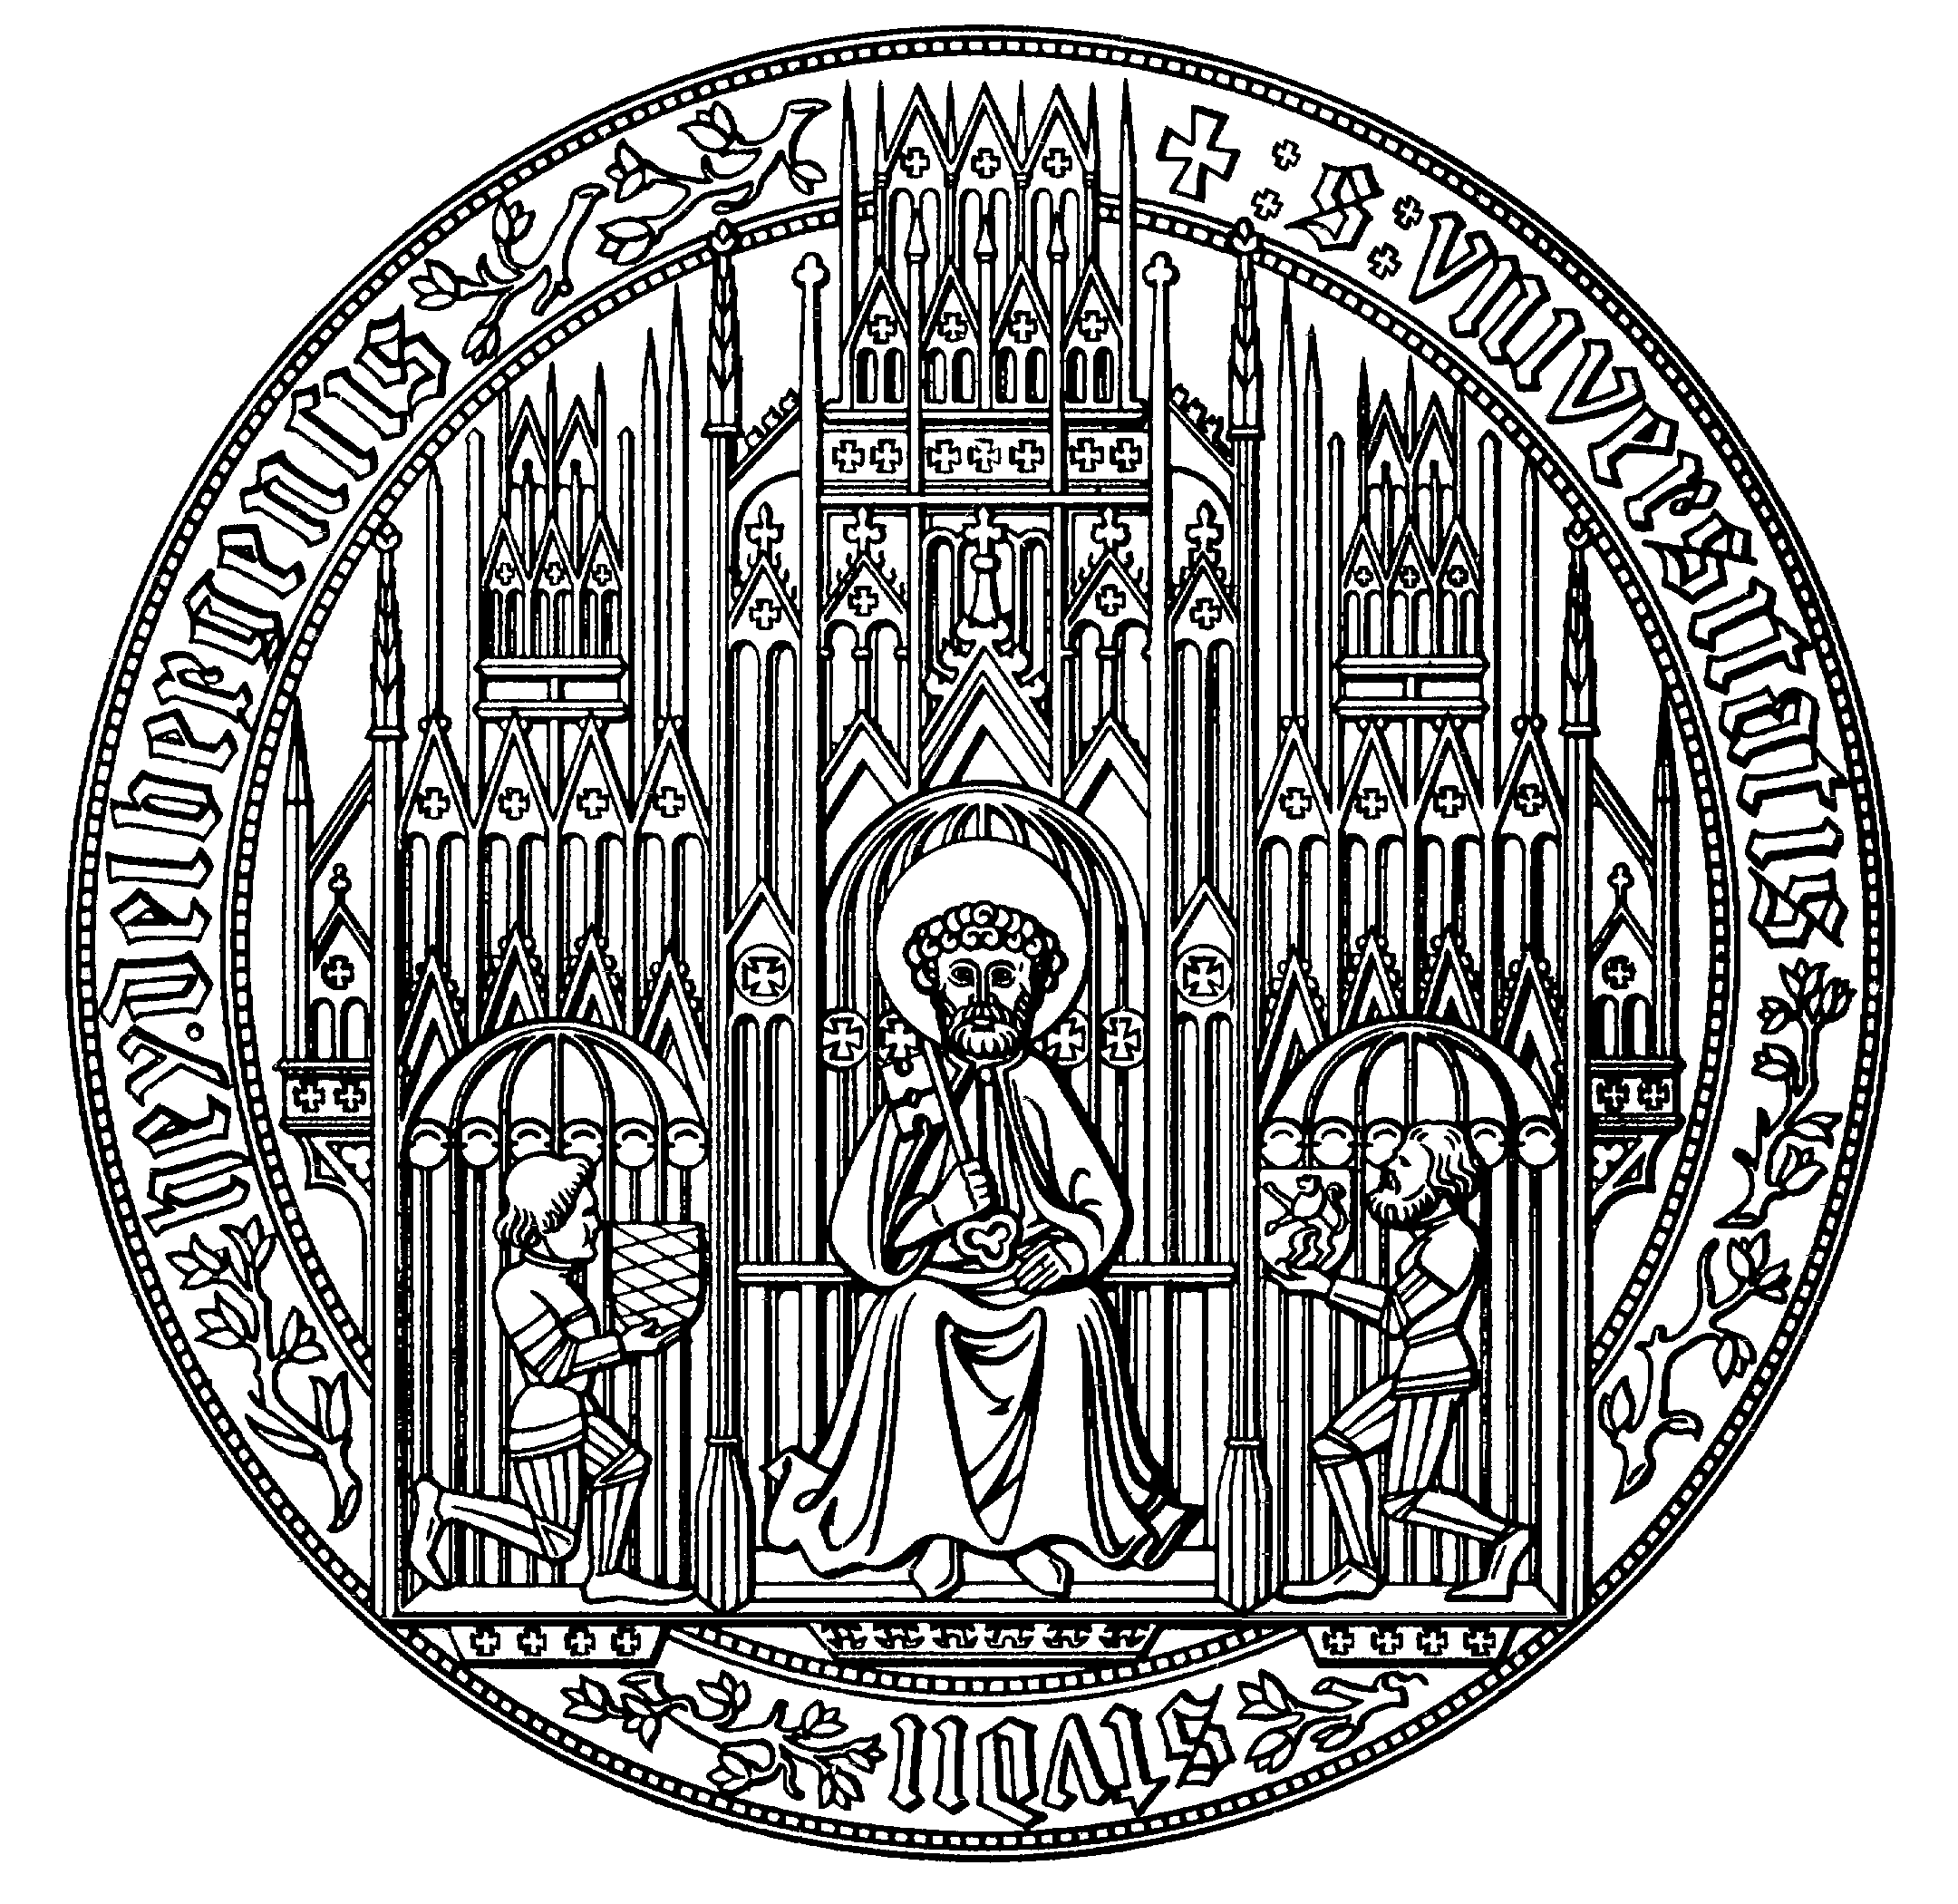
\includegraphics[width=5cm]{UniHD.png}

\end{center}

\newpage
\setcounter{page}{1}		% set page count to start with 1 here

\section*{Nomenclature}
The files supplied with this document are named with the following suffixes:
\begin{table}[h!]
\begin{tabular}{ll}\toprule
suffix          & meaning \\ \midrule
\verb+-b+       & bias corrected \\
\verb+-bf+      & bias and flatfield corrected	\\
\verb+-bsf+     & as -bf but scaled by the factor stored in factors.txt	\\
\verb+-bff+     & as -bf with substracted fringe pattern (no masking applied)	\\
\verb+-bffm+    & as -bf with substracted fringe pattern (masking applied)	\\
\verb+-bffg{5-20}+    & as -bff with gaussian kernel of size \verb+{5-20}+ applied	\\
\verb+-bffu{5-20}+    & as -bff and unsharp masked with a gaussian kernel of size \verb+{5-20}+	\\
\bottomrule
\end{tabular}
\end{table}

\section*{Demanded files}
In the archive \verb+files.zip+, together with this \verb+.pdf+ and some other
files to eliminate possible misunderstandings we supply these files as
requested in the exercise:
\begin{table}[h!]
\begin{tabular}{p{4cm}l}\toprule
name                        & file         \\ \midrule
\verb+fringe.fits+          & FITS image of the pure fringe pattern \\
\verb+science6-bff.fits+    & final reduced FITS image of the object science6 \\
\verb+science6-bffu10.fits+ 
and figure \ref{fig:gs} 
(top right)                 & file of the unsharp mask image for question B\\
\verb+fringe_mask.fits+     & re-reduced FITS image of science6 for question C	\\
\bottomrule
\end{tabular}
\end{table}

\section*{Exercise A.}

\begin{listing}[h!]
\begin{minted}{shell}
ecl> imarith @science-bf.txt * @factors.txt  @science-bfs.txt
ecl> imcombine @science-bfs.txt fringe.fits combine=median

ecl> imarith fringe.fits / @factors.txt  @scaled_fringes.txt
ecl> imarith @science-bf.txt - @scaled_fringes.txt @science-bff.txt
\end{minted}
\caption{Operations executed in IRAF for exercise A.}
\label{fig:ca}
\end{listing}

We used the bias and flatfield corrected images \verb+science[1-7].fits+ from
the lecture for this exercise. Their names are stored in a file named 
\verb+science-bf.txt+.

To combine the images for generating the pure fringe pattern, we calculate their
respective correction factors by looking at regions roughly in the same area
of the images where there are no stars or other foreground objects visible.
See figure \ref{fig:reg}.

\begin{figure}[h!]
\centering
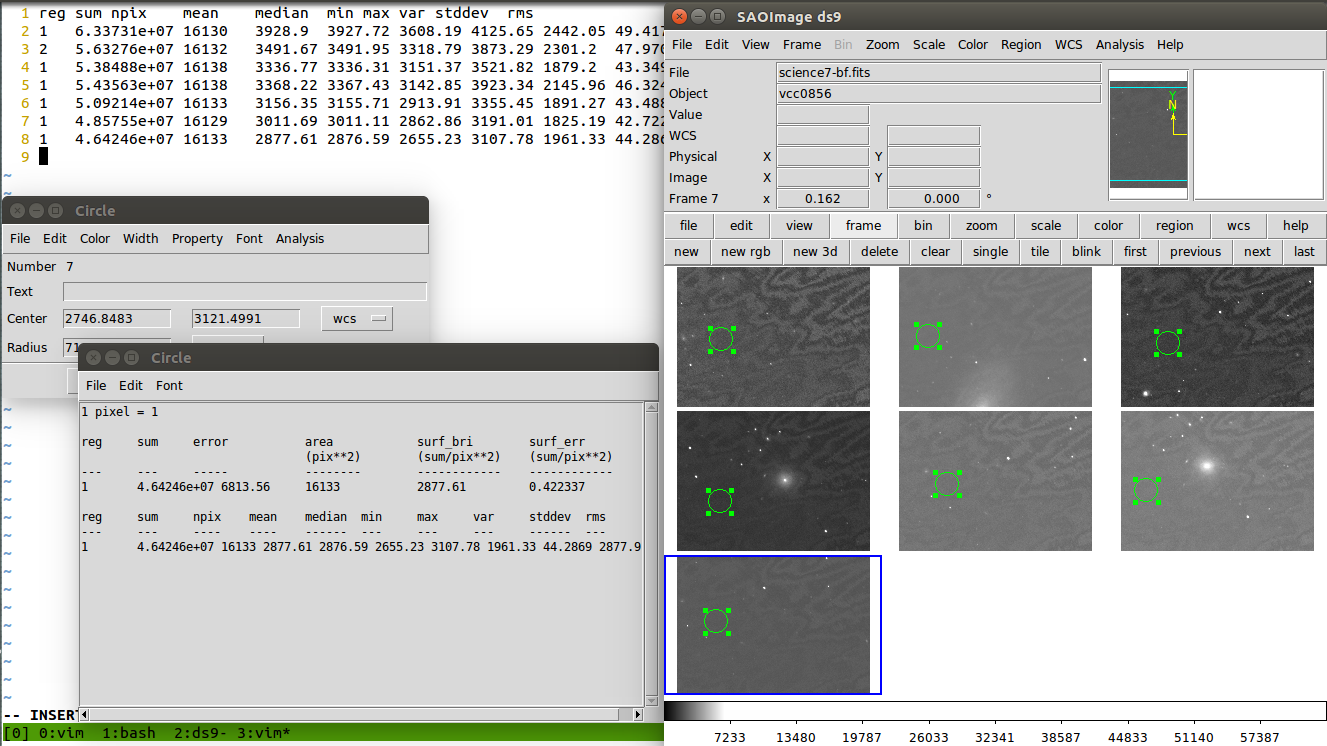
\includegraphics[width=\linewidth]{../pic/regions}
\caption{Regions analysed for getting the sky counts of each science picture.}
\label{fig:reg}
\end{figure}

Next we take the median counts $I_{sky,\,i}$ from each region and store them.
As refence picture we take \verb+science6.fits+ with the sky count $I_{sky,\,ref}$.
The correction factors $f_i$ are the simply calculated via
\begin{align}
    f_i &= \frac{I_{sky,\,ref}}{I_{sky,\,i}} .
\end{align}

Now we multiply each image $i$ with its respective factor and store them
according to names we specified in the file \verb+science-bfs.txt+.
See line 1 in listing \ref{fig:ca}. The fringe pattern is then generated
by combining these images using the \verb+median+ method and stored in the
file \verb+fringe.fits+. See line 2 in listing \ref{fig:ca}. To test if the
pattern resembles the one we see in our original image we compare pattern
and original in figure \ref{fig:fr}. It matches extremely well.

\begin{figure}[h!]
\centering
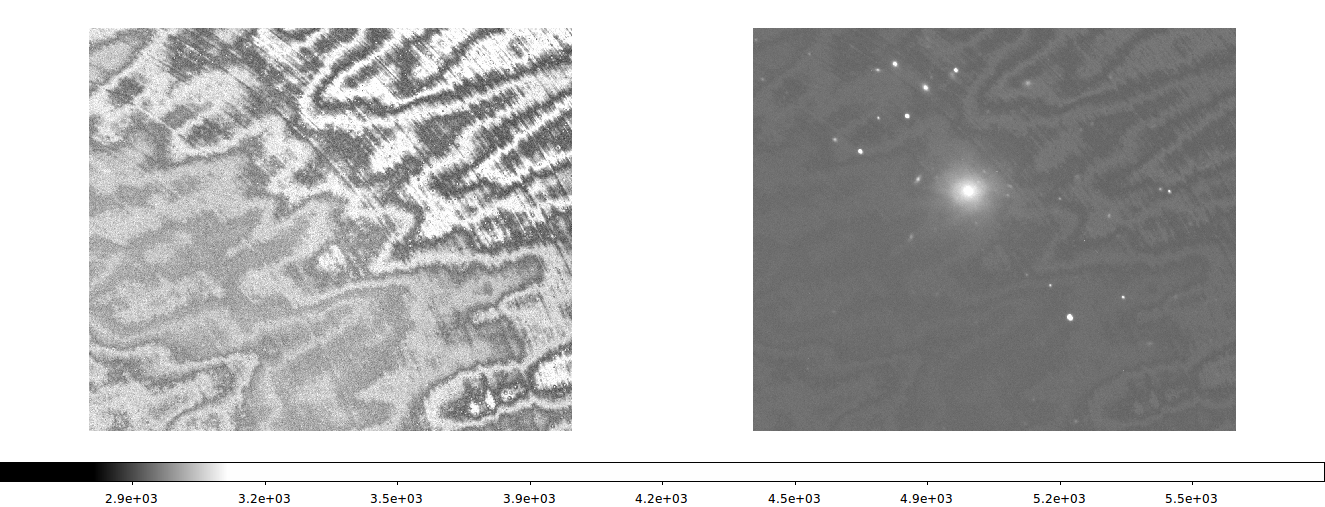
\includegraphics[width=\linewidth]{../pic/fringes}

\caption{Left: Fringe pattern generated as described in Task A. Right:
         Original image for comparison.}
\label{fig:fr}
\end{figure}

Finally, to correct the images, we divide the fringe pattern by the corresponding
factors and substract the generated pattern from each image, as done in lines
4 and 5 in listing \ref{fig:ca}.

The resulting image generated from \verb+science6-bf.fits+ can be found in figure
\ref{fig:res} and supplied with this sheet as \verb+science6-bff.fits+.

\begin{figure}[h!]
\centering
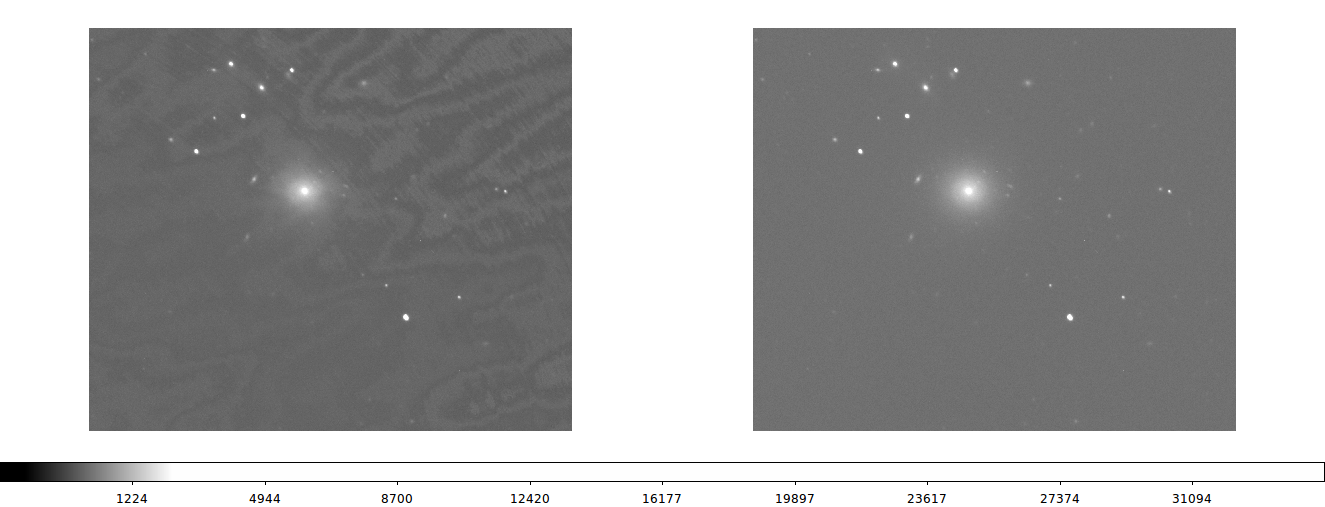
\includegraphics[width=\linewidth]{../pic/fringe-noFringe}
\caption{Left: Original image. Right: Fring substracted image.}
\label{fig:res}
\end{figure}


            %======================================%
            %==      TODO: INTERPRETATION        ==%
            %======================================%


\section*{Exercise B.}

\begin{listing}[h!]
\begin{minted}{shell}
# Repeat for sigma=15 and 20
ecl> gauss science6-bff.fits science6-bffg10.fits sigma=10
ecl> imarith science6-bff.fits / science6-bffg10.fits science6-bffu10.fits
\end{minted}
\caption{Operations executed in IRAF for exercise B.}
\label{fig:cb}
\end{listing}

For our gaussian kernel we chose a $\sigma$ in the range of
\SIrange{5}{20}{\pixel}. As we are interested in features of size
\SIrange{1}{2}{\arcsecond} and the image scale is given as 
\SI{0.24}{\arcsecond\per\pixel}, this results in an area of interest of about 
\SIrange{4}{8}{\pixel}.
The resulting unsharp masked image can be found in figure \ref{fig:gs}. Each
image has been optimized to show maximum contrast while still showing all the
visible structures well. One can see, that for $\sigma = 10$ the spiral arms
are nicely visible, while the core is not blurred out to much, as is the case
with $\sigma = 15$ and $20$. With $\sigma = 5$ the noise in the image dominates
the spiral arms.

\begin{figure}
\centering
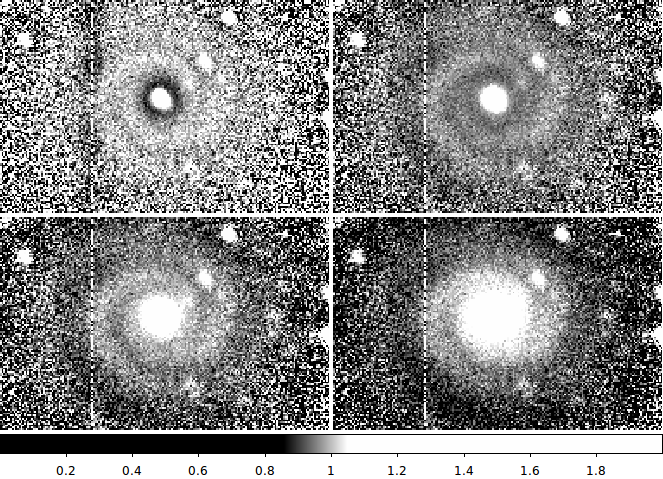
\includegraphics[width=\linewidth]{../pic/gauss}
\caption{   Unsharp masked images using different kernel sizes using different kernel sizes.
            From top left, clockwise: $\sigma= \{5,10,15,20\}$.}
\label{fig:gs}
\end{figure}

\section*{Exercise C.}

\begin{listing}[h!]
\begin{minted}{shell}
# for image 1-7:
ecl> hedit science1-bf.fits mymask masks/objectmask1.fits add=yes verify=no
ecl> imcombine @science-bfs.txt fringe_mask.fits combine=median masktype=!mymask

ecl> imarith fringe_mask.fits / @factors.txt  @scaled_fringes-m.txt
ecl> imarith @science-bf.txt - @scaled_fringes-m.txt @science-bffm.txt
\end{minted}
\caption{Operations executed in IRAF for exercise C.}
\label{fig:cc}
\end{listing}

After updating the header as can be seen in line 1 in listing \ref{fig:cc}
we calculate the fringe pattern now without the objects, exactly as in 
exercise A (lines 2-5 in listing \ref{fig:cc}).

As the resulting fringe pattern is extremely similar to the one we calculated
before, we also calculate the difference between the two. The result is shown
in figure \ref{fig:df} on the top. This difference pattern can then also be
observed, when looking at the differences in the resulting image
\verb+science6-bffm.fits+ after substracting the fringe pattern (figure
\ref{fig:df} bottom).

\begin{figure}
\centering
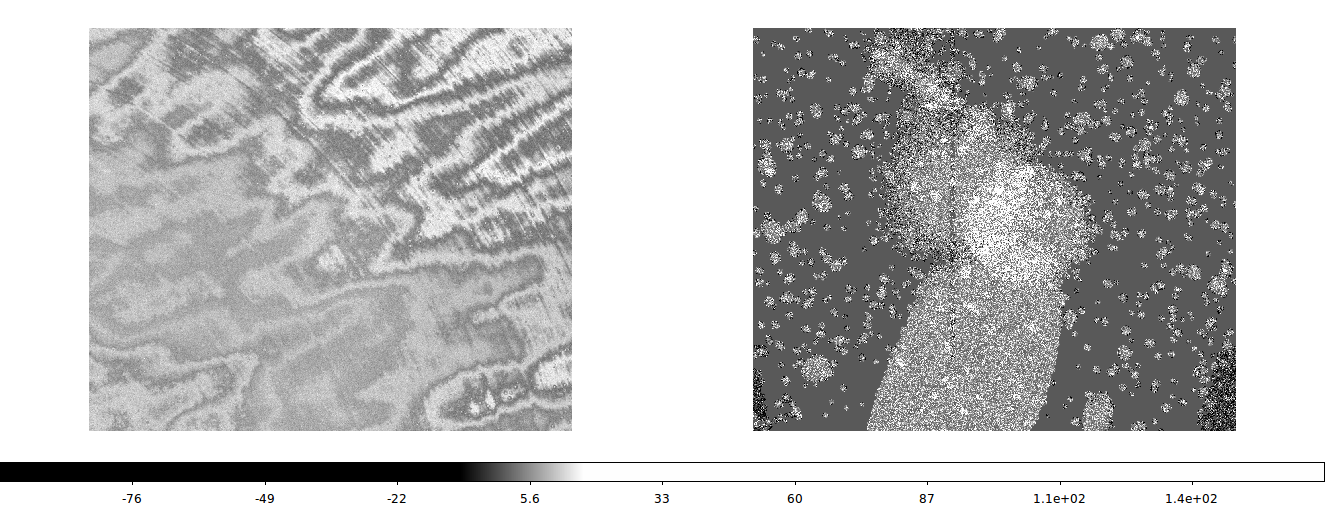
\includegraphics[width=\linewidth]{./pic/diff_fringe}
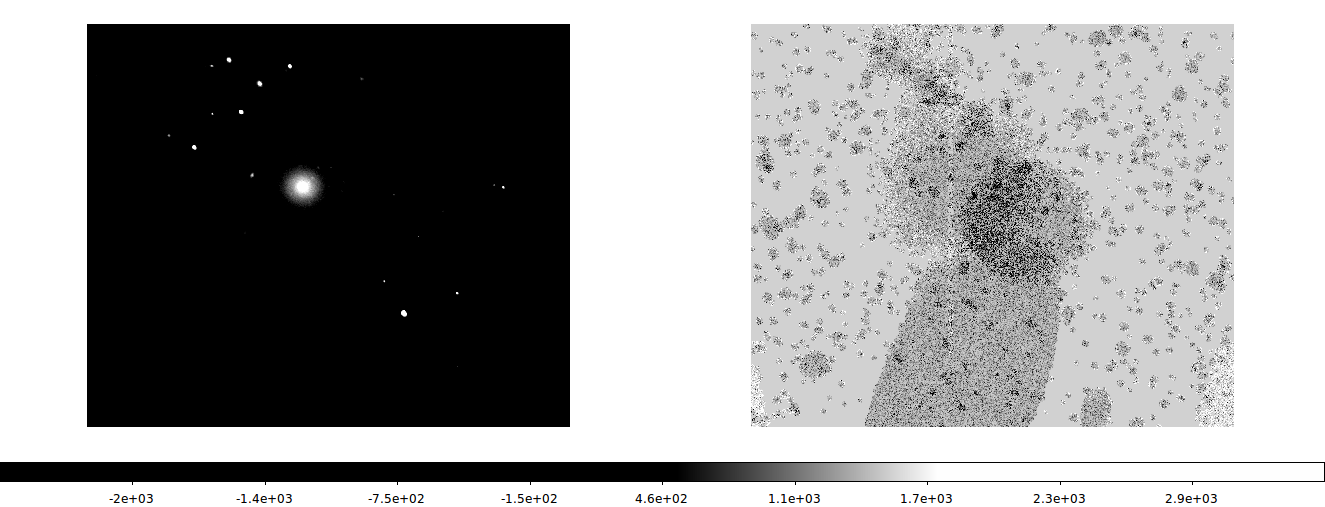
\includegraphics[width=\linewidth]{./pic/diff_result}
\caption{Results using the newly accomplished version of the fringe pattern (left)
        and differences (right) to the results using the old version. The differences
        are relatively small, compared to the dynamic range of the image ($\sim
        100$ vs $\sim 100000$).}
\label{fig:df}
\end{figure}

The differences are extremely small. They are in the range of -100 to 100 counts
while the dynamic range of the picture spans a range of $\approx 10000$ counts.

\end{document}
